\documentclass[handout,t]{beamer}
\usepackage{graphicx,url}
\usepackage{inputenc}
% \usepackage[english]{babel}
\batchmode
\usepackage{amsmath,amssymb,enumerate,epsfig,bbm,calc,color,ifthen,capt-of}
% \usepackage{xepersian}
% \settextfont{XB Niloofar}

\usetheme{Darmstadt}
\usecolortheme{wolverine}

%-----Title,authors,addressed to:..------------
\title[Topic]{Title and topic}
\author[if you want put here who aro you going to present or the name organization]
{author 1 \texttt{email1@domain.com} \\author 2 \texttt{email2@domain.com}\\}
\date{\today}
%--------Logo from the slides at the bottom right
\pgfdeclareimage[height=1cm]{IUST}{../figures/logo.pdf}
\logo{\pgfuseimage{IUST}\hspace*{0.5cm}}
%------------Menú en la parte superior de la diapositiva(linkeado)
\AtBeginSection[]
{
  \begin{frame}<beamer>
    \frametitle{Outline}
    \tableofcontents[currentsection]
  \end{frame}
}
\beamerdefaultoverlayspecification{<+->}
%\usepackage[height=30cm,a5paper,hmargin={3cm,3cm}]{geometry}
\setbeamersize{text margin left=1cm,text margin right=1cm}
%%%-------------BEGIN DOCUMENT--------%%%%%
\begin{document}
% \setbeamertemplate{navigation symbols}{[default]{}}%navegaton bar
% \setbeamertemplate{navigation symbols}{}%navegaton bar
\setbeamertemplate{footline}[frame number]
\setbeamertemplate{page number in head/foot}[totalframenumber]

%If we want the parts that have not yet appeared in our sequence to appear transparently, in the preamble we add:
\setbeamercovered{transparent}
%----------Index--------------
\frame{\titlepage}
\section[]{}
\begin{frame}{Index}
  \tableofcontents
\end{frame}
%----------- End Index
%----Introduction----
\section{Introduccion}
\begin{frame}{Introduccion}
	Introduccion aca
\end{frame}

\begin{frame}{Spin Current}
	\begin{figure}[!ht]
		\centering
		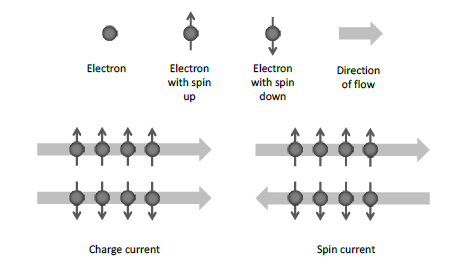
\includegraphics[width=0.7\linewidth]{../figures/spinchargecurent.png}
		\label{fig:spinchargecurent}
	\end{figure}
\end{frame}

\begin{frame}{MOSFET}
	\begin{figure}[!ht]
		\centering
		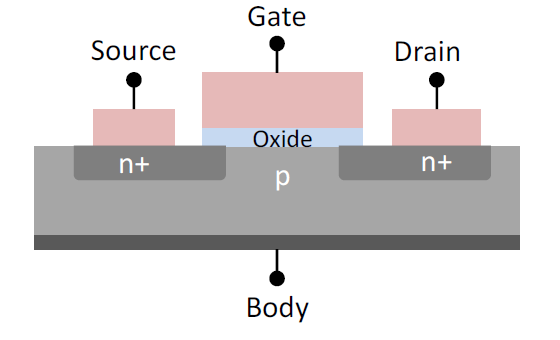
\includegraphics[width= 0.8\linewidth]{../figures/MOSFET.png}
		\label{fig:mosfet}
	\end{figure}
\end{frame}
\begin{frame}{GrapheneFET}
	\begin{figure}[!ht]
		\centering
		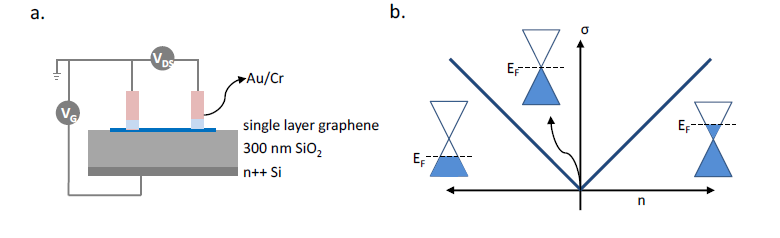
\includegraphics[width=\linewidth]{../figures/GrapheneFET.png}
		\label{fig:graphenefet}
	\end{figure}
\end{frame}
\begin{frame}{Spin Injections}
	\begin{figure}[!ht]
		\centering
		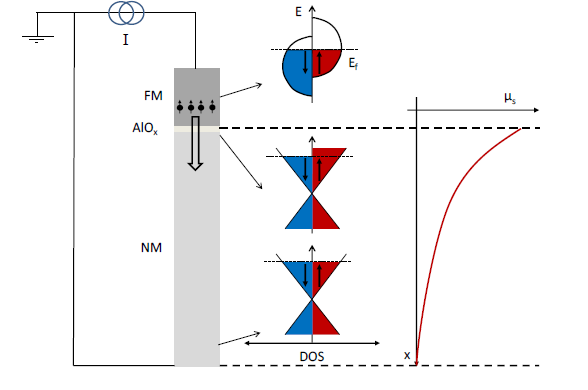
\includegraphics[width=\linewidth]{../figures/spininjection.png}
		\label{fig:spininjection}
	\end{figure}
\end{frame}
\begin{frame}{Two channel}
	\begin{figure}[!ht]
		\centering
		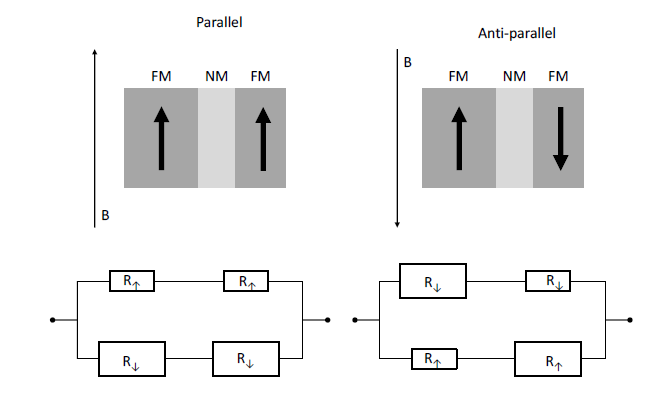
\includegraphics[width=\linewidth]{../figures/twochannelmodel.png}
		\label{fig:twochannelmodel}
	\end{figure}
\end{frame}
%-----end Introduction
%---begin section-------
\section{Borophene}
\begin{frame}{text here}
	text here
\end{frame}
%---begin subsection----
\subsection{text here}
\begin{frame}{borophenedev}
	\begin{figure}[!h]
		\centering
		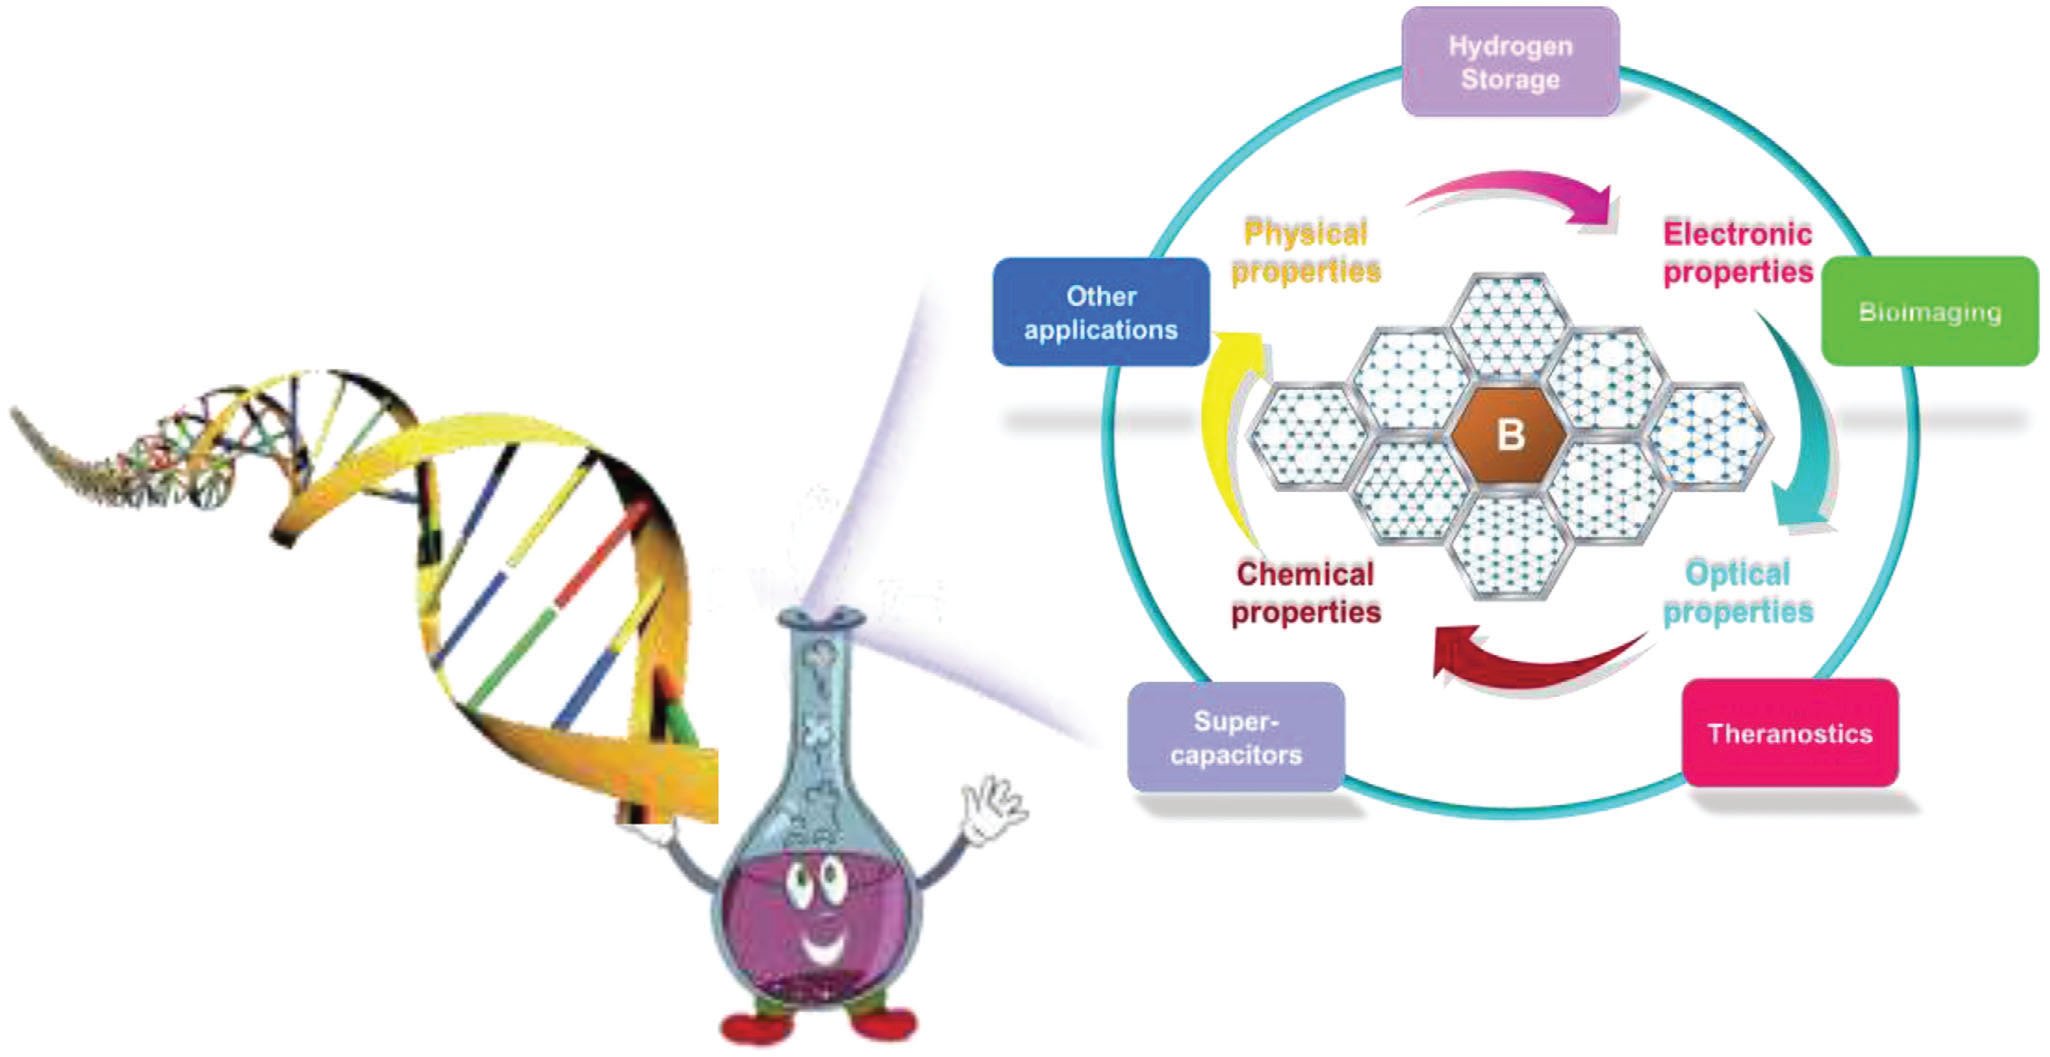
\includegraphics[width=\linewidth]{../figures/borophenedev.png}
		\label{fig:borophenedev}
	\end{figure}
\end{frame}
%end subsection
%---begin subsection----
\subsection{theory borophene}
\begin{frame}{theoryborophene}
	\begin{figure}
		\centering
		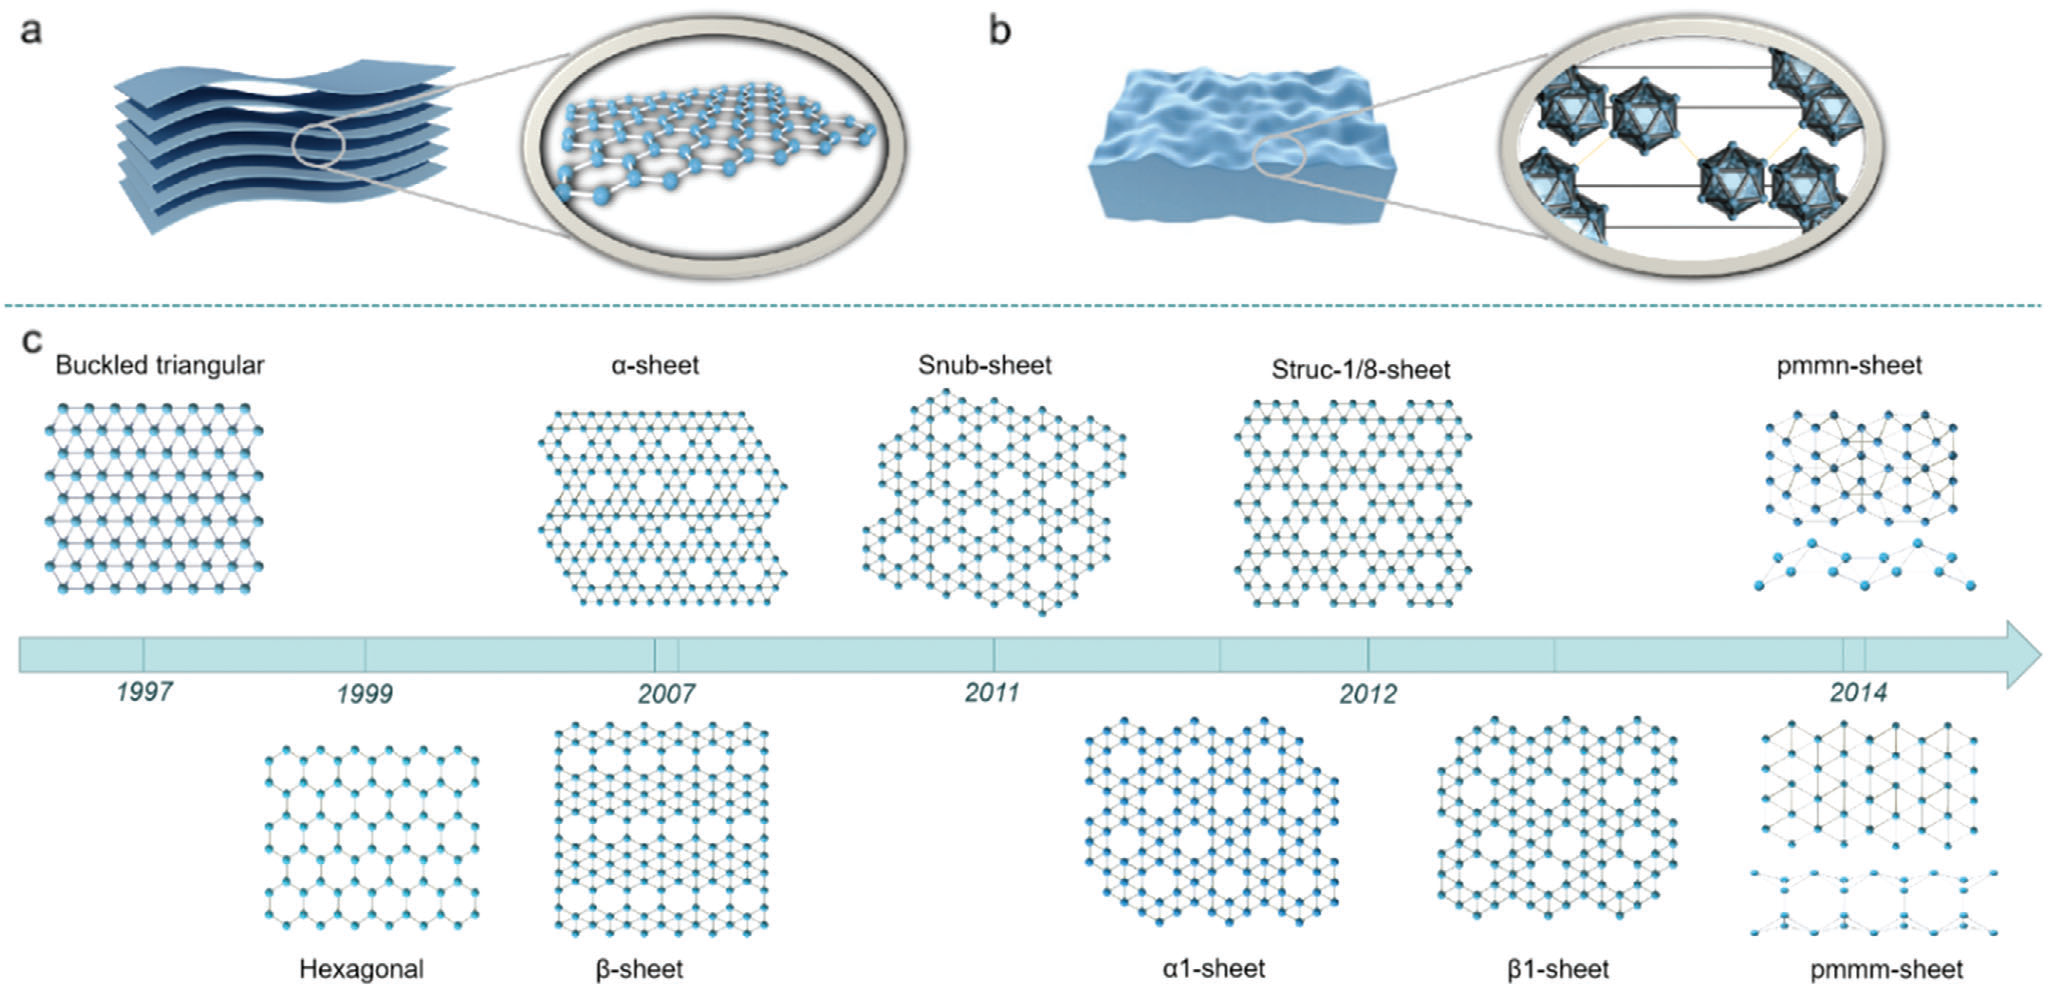
\includegraphics[width=\textwidth]{../figures/theory-borophene.png}
		\label{theoryborophene}
	\end{figure}
\end{frame}
%end subsection
%---begin subsection----
\subsection{electrical properties}
\begin{frame}{electricalproperties}
	\begin{figure}
		\centering
		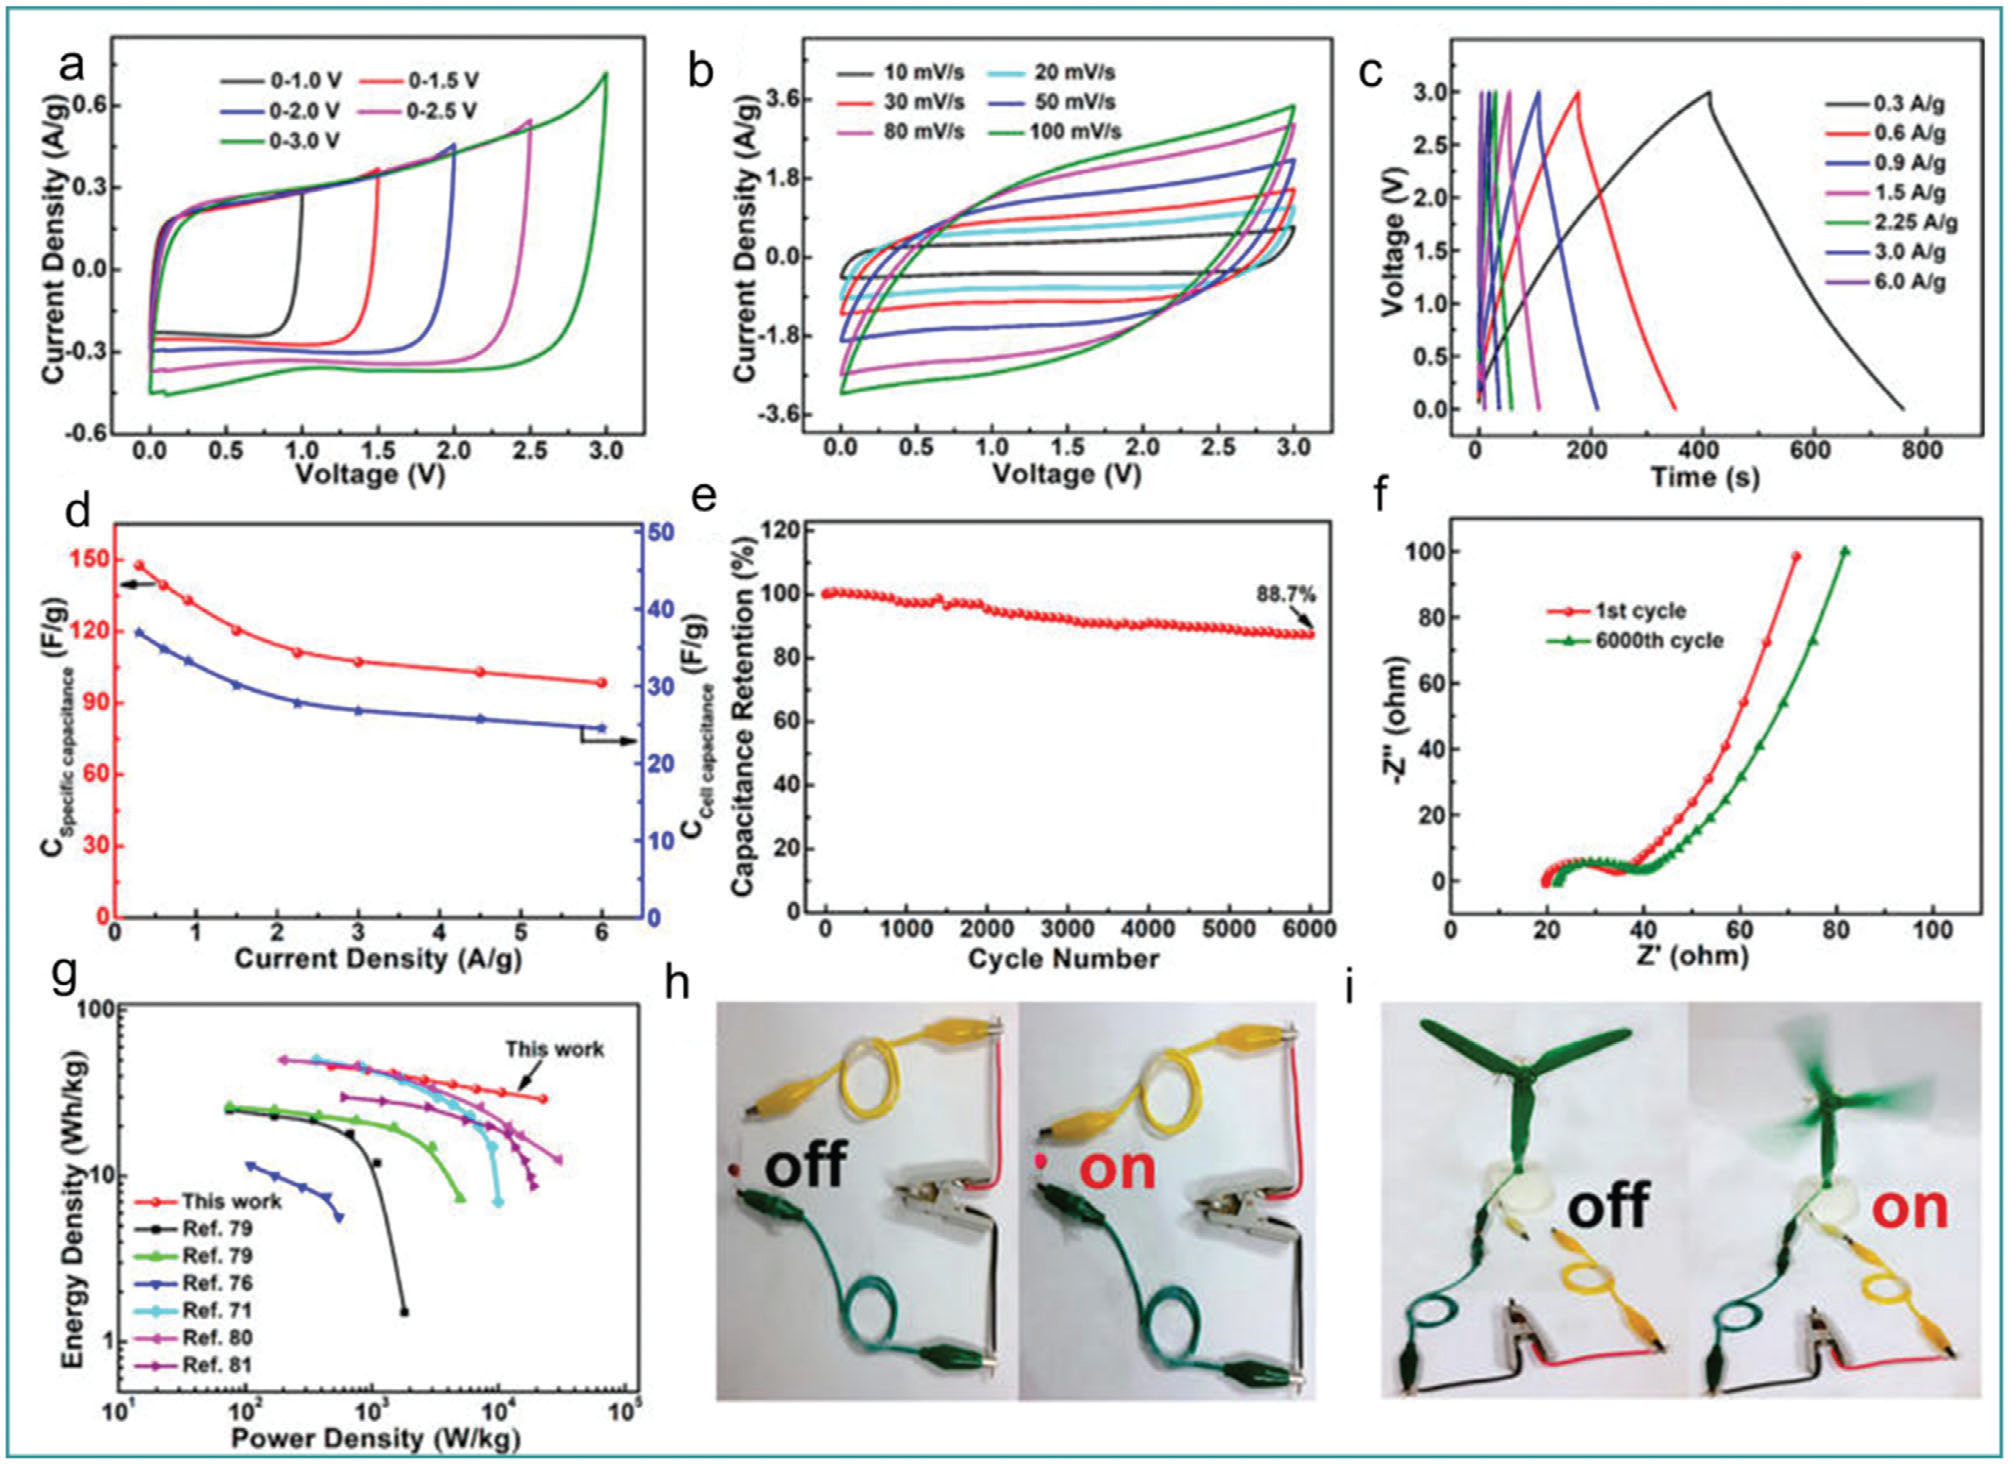
\includegraphics[width=0.5\linewidth]{../figures/electricalproperties.png}
		\label{fig:electricalproperties}
	\end{figure}
\end{frame}
%end subsection
%---begin subsection----
\subsection{absorbtion}
\begin{frame}{absorbtion}
	\begin{figure}
		\centering
		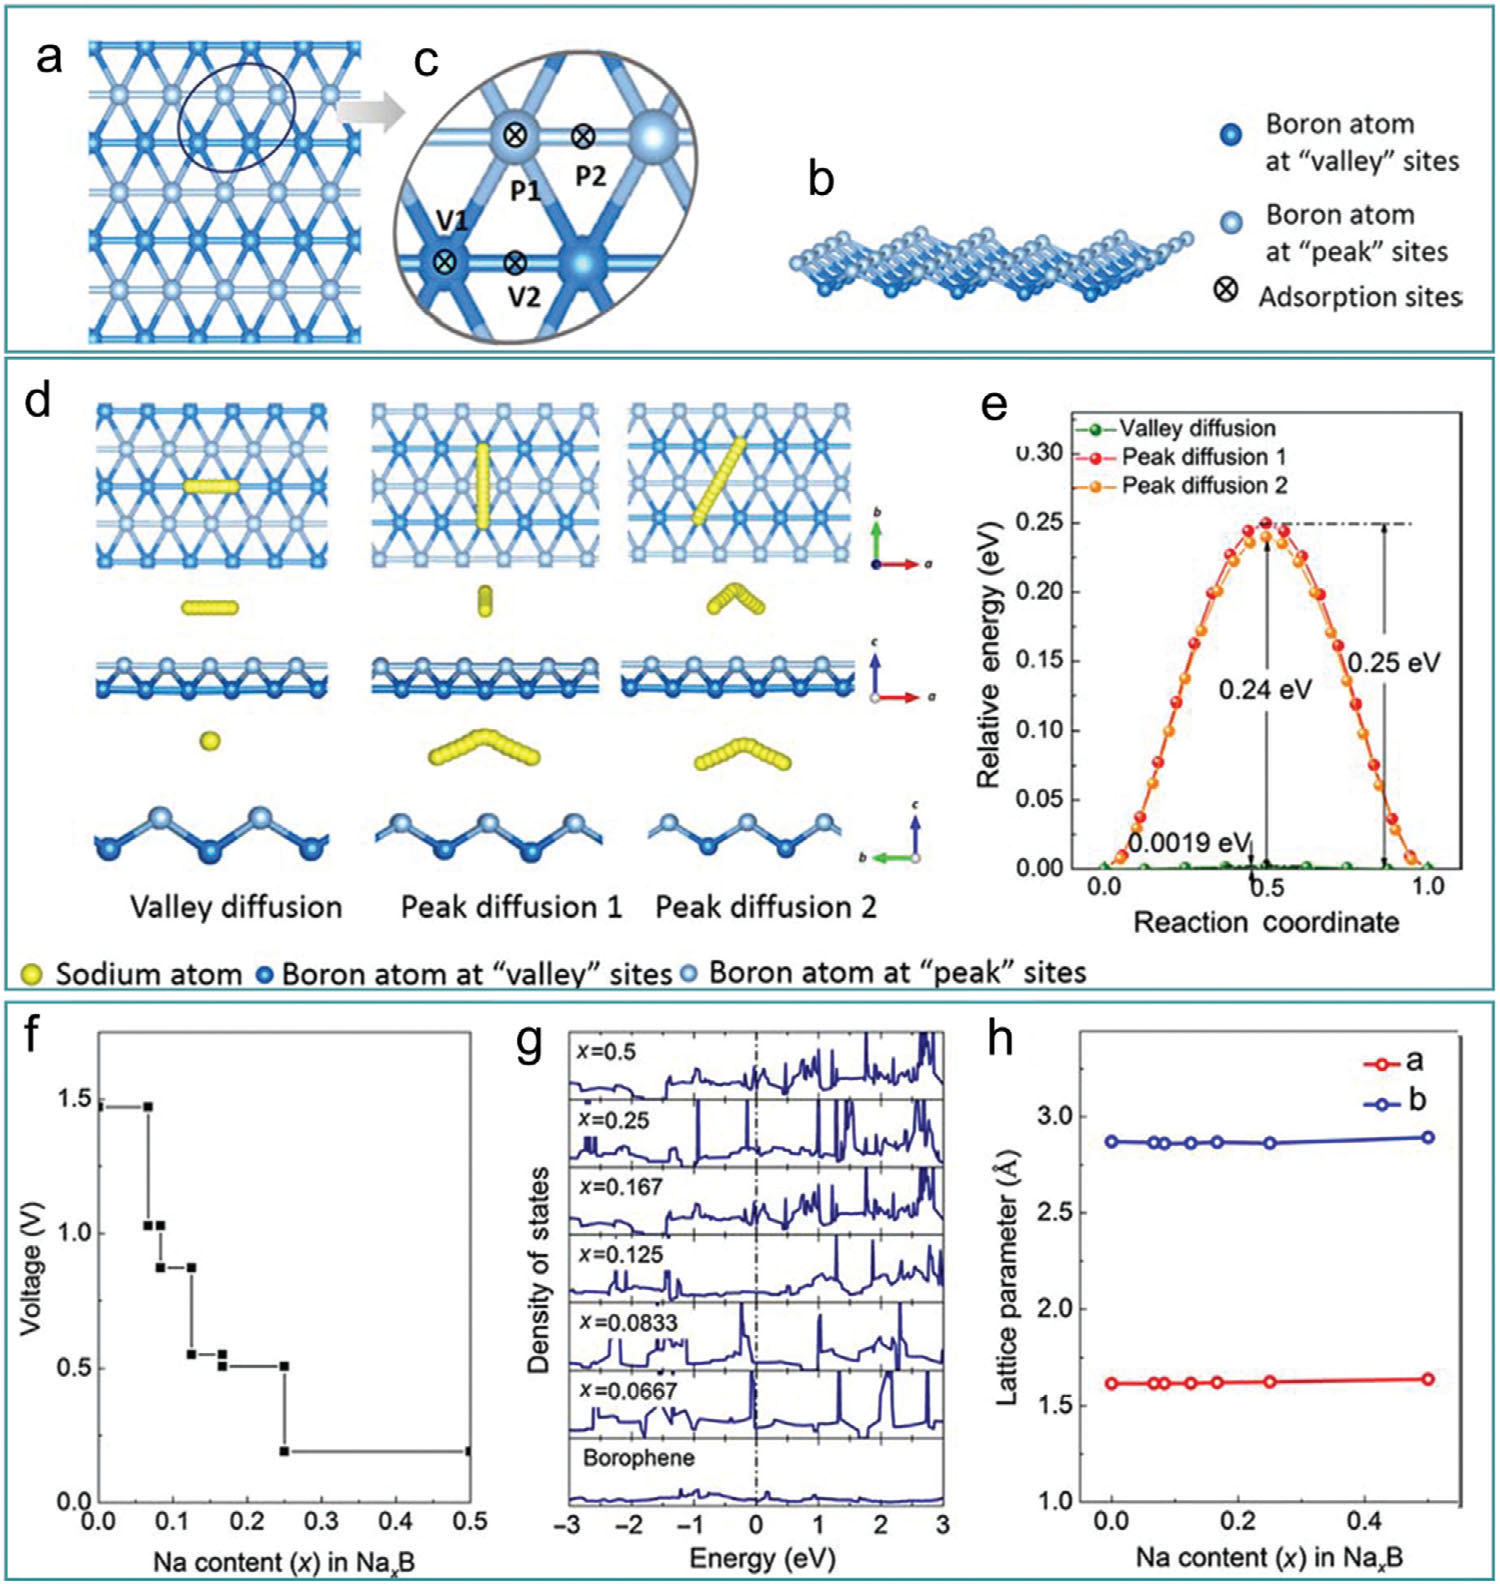
\includegraphics[width=0.5\linewidth]{../figures/absorbtion.png}
		\label{fig:absorbtion}
	\end{figure}
\end{frame}
%end subsection
%---begin subsection----
\subsection{alphasheet}
\begin{frame}{alphasheet}
	\begin{figure}
		\centering
		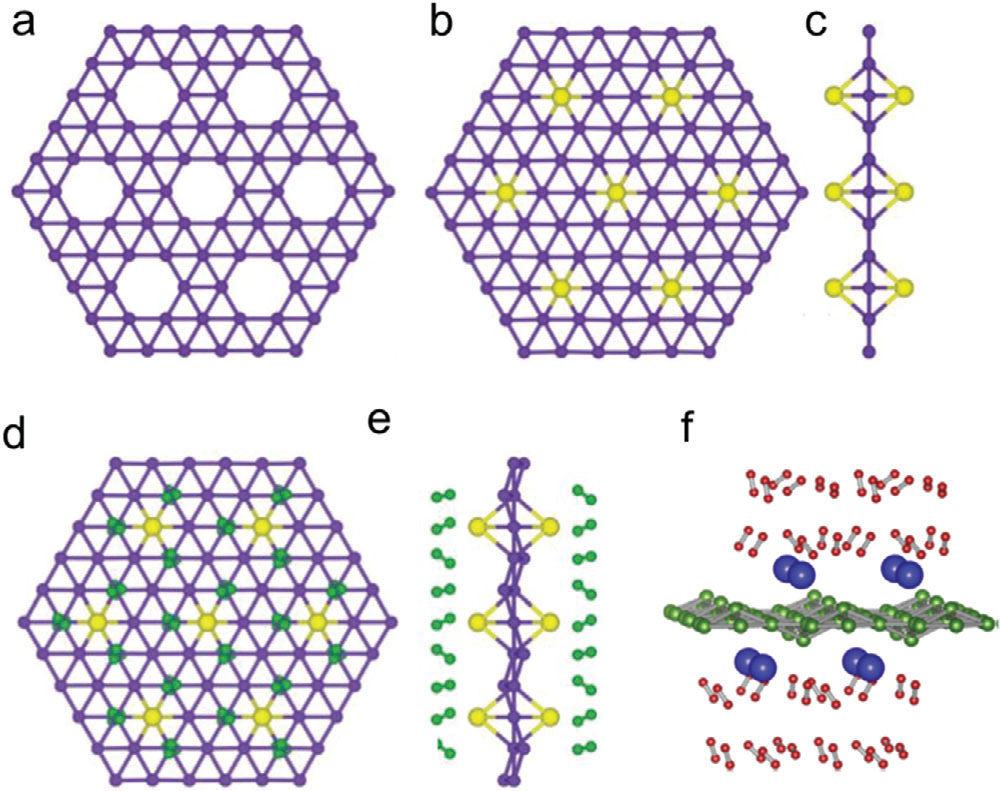
\includegraphics[width=0.5\linewidth]{../figures/alphasheet.png}
		\label{fig:alphasheet}
	\end{figure}
\end{frame}
%end subsection
\subsection{Multimodal}
\begin{frame}{Multimodal}
	teest
	\begin{figure}
		\centering
		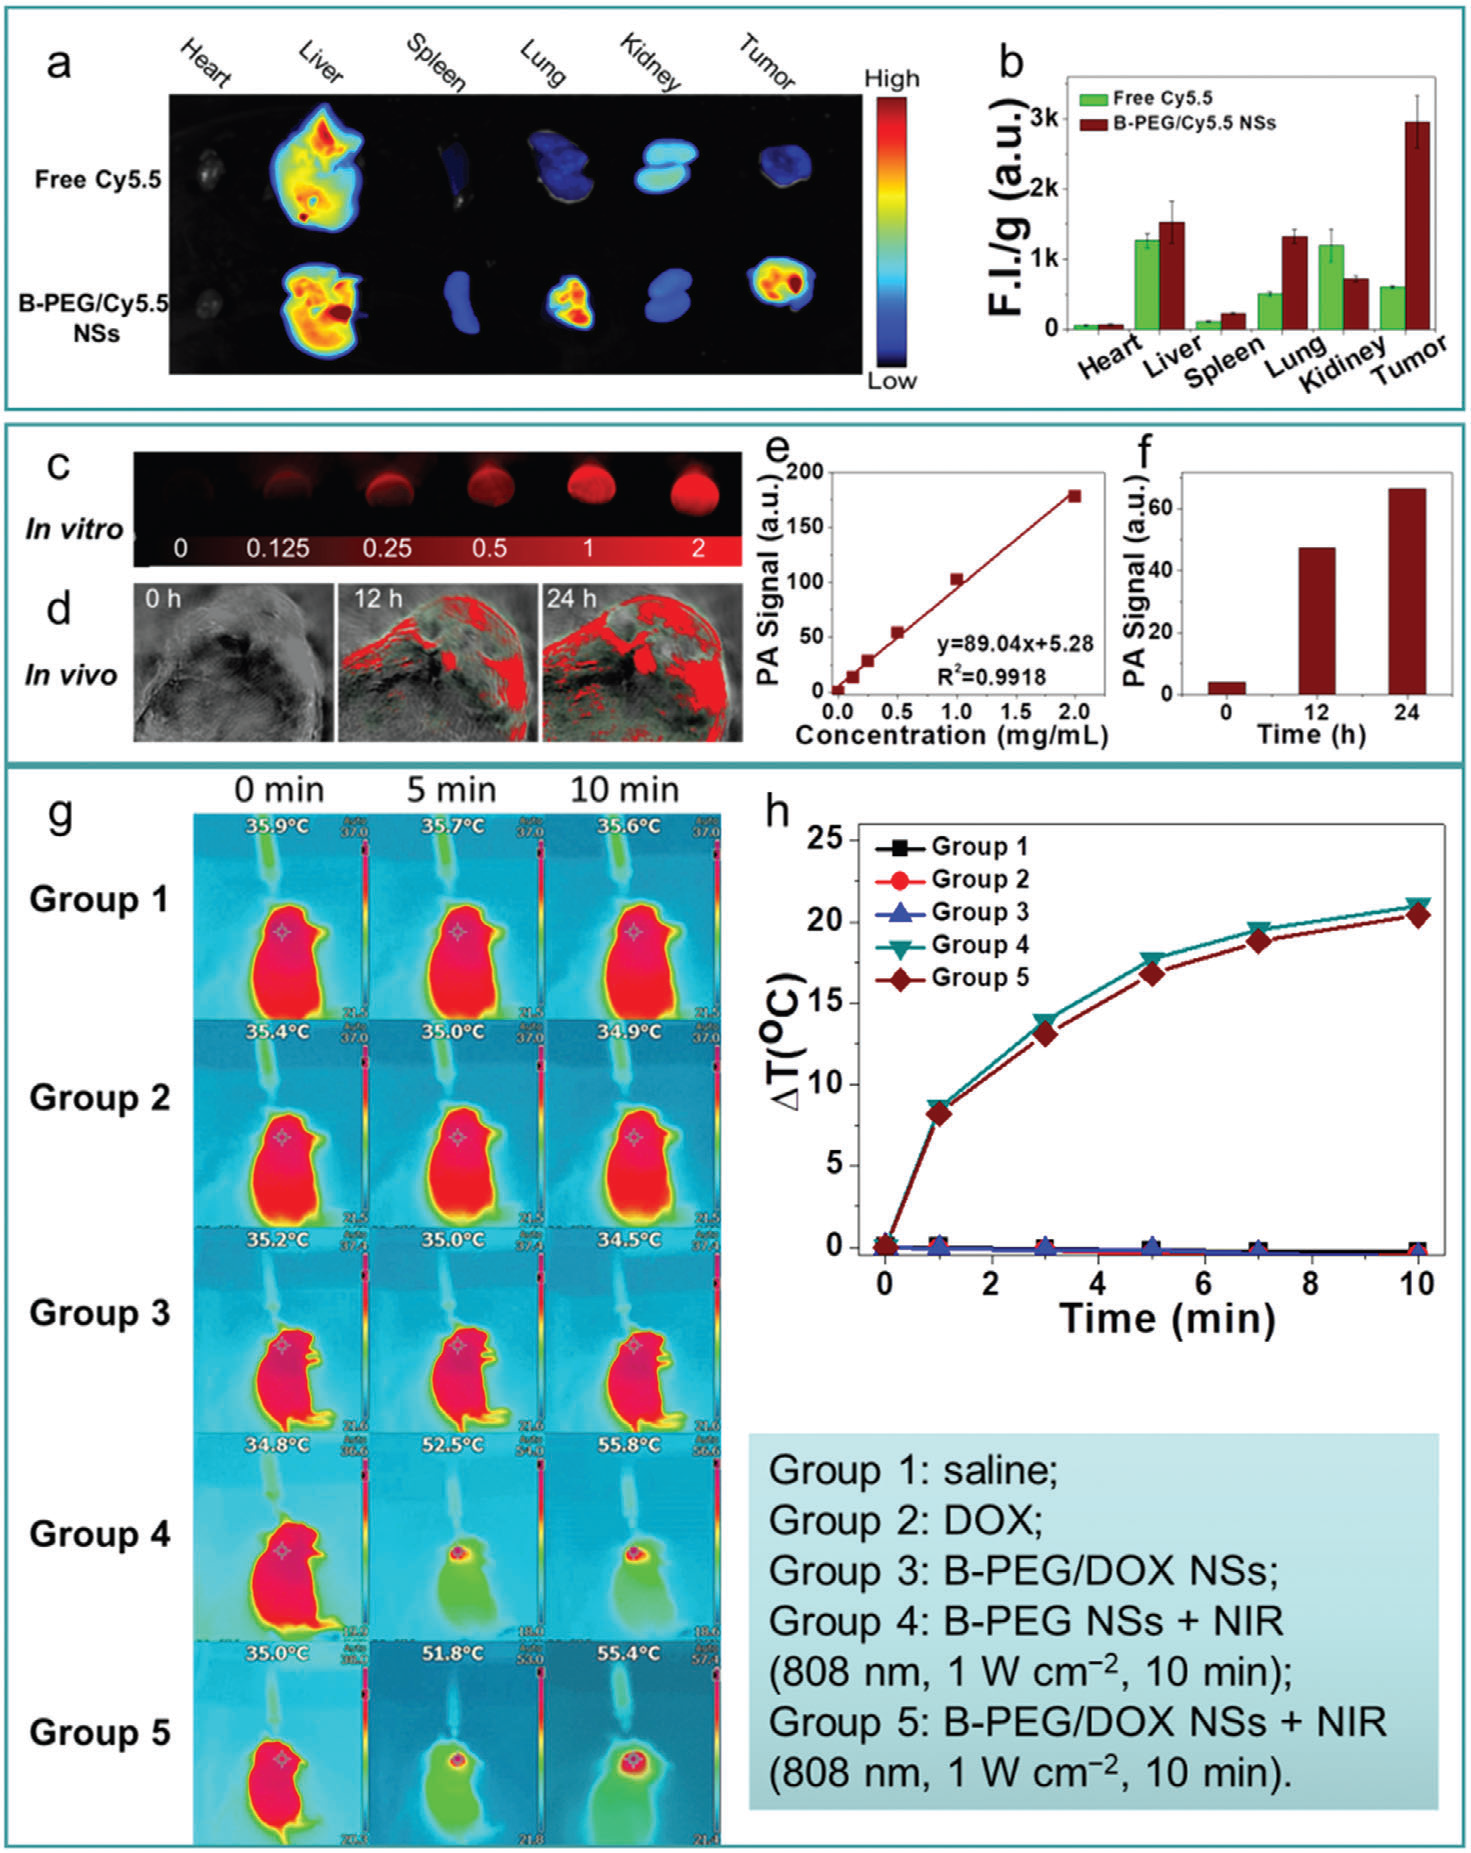
\includegraphics[width=0.5\linewidth]{../figures/Multimodal.png}
		\label{fig:Multimodal}
	\end{figure}
\end{frame}
%end subsection
\subsection{UV}
\begin{frame}{UV}
	teest
	\begin{figure}
		\centering
		\includegraphics[width=0.5\linewidth]{../figures/UV.png}
		\label{fig:UV}
	\end{figure}
\end{frame}
%end subsection
%end subsection
\subsection{Diraccone}
\begin{frame}{Diraccone}
	teest
	\begin{figure}
		\centering
		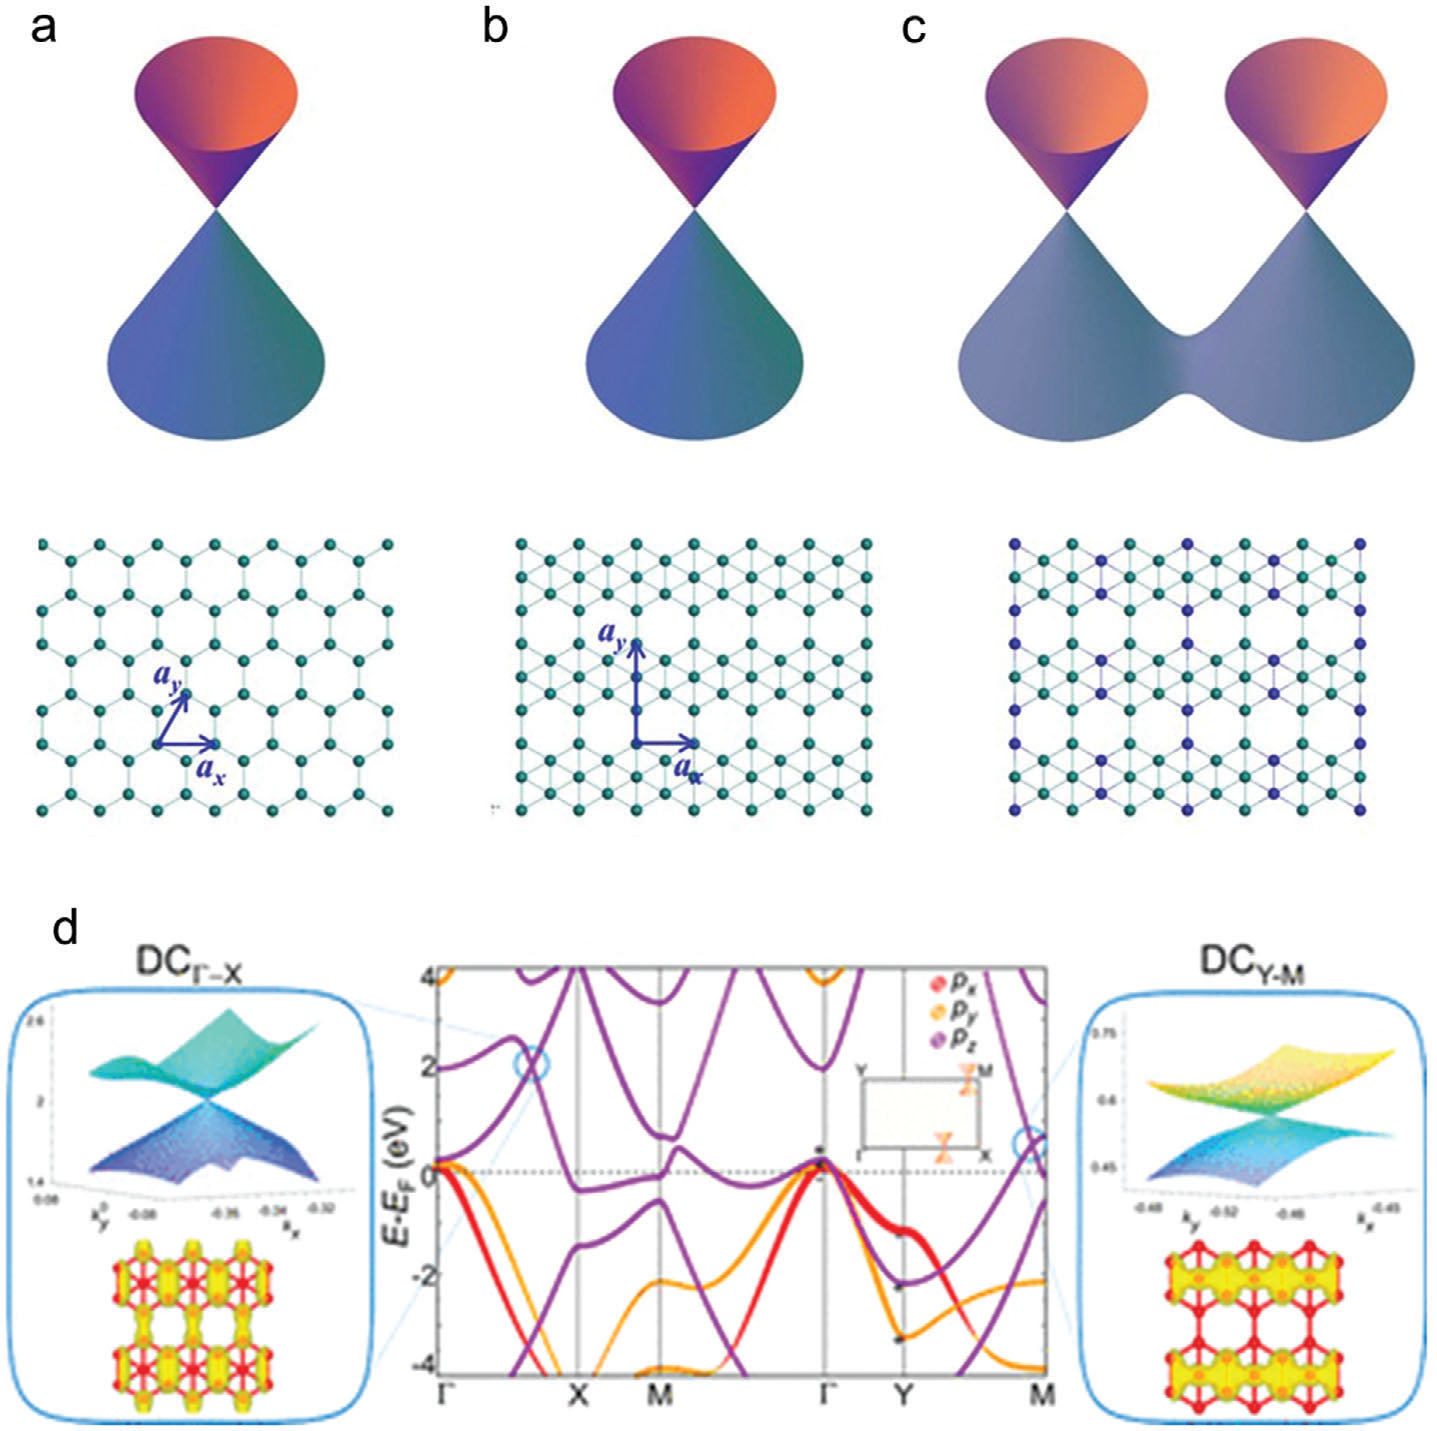
\includegraphics[width=0.5\linewidth]{../figures/Diraccone.png}
	\end{figure}
\end{frame}
%end subsection
%---end section----
%---begin section-------
\section{Methodes}
\begin{frame}{Mode Matching}
	\begin{figure}
		\centering
		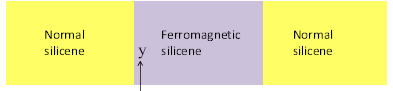
\includegraphics[width=\linewidth]{../figures/vallyschmatic.png}
		\label{fig:vallyschmatic}
	\end{figure}
\end{frame}
%---end section----
\begin{frame}{NEGF}
	\begin{figure}
    \centering
    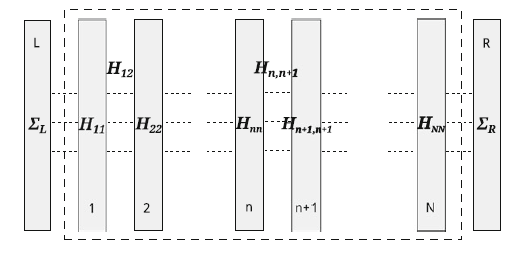
\includegraphics[width=0.25\linewidth]{../figures/iteration.png}
    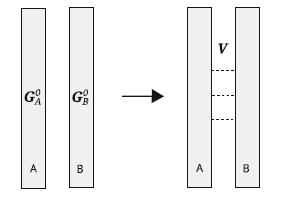
\includegraphics[width=0.25\linewidth]{../figures/greendyson.png}
    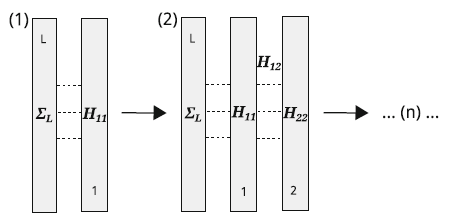
\includegraphics[width=0.25\linewidth]{../figures/iterationchannelgreen.png}
    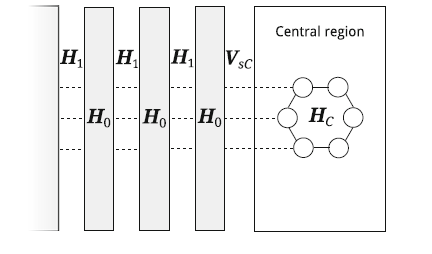
\includegraphics[width=0.25\linewidth]{../figures/leaditerationgreen.png}
    \label{fig:greendyson}
\end{figure}
ttttttt
\begin{equation}
    \left( \begin{matrix}
           {{G}_{A}} & {{G}_{AB}}  \\
           {{G}_{BA}} & {{G}_{B}}  \\
        \end{matrix} \right)=\left( \begin{matrix}
           G_{A}^{0} & 0  \\
           0 & G_{B}^{0}  \\
        \end{matrix} \right)+\left( \begin{matrix}
           G_{A}^{0} & 0  \\
           0 & G_{B}^{0}  \\
        \end{matrix} \right)\left( \begin{matrix}
           0 & {{V}_{AB}}  \\
           {{V}_{AB}} & 0  \\
        \end{matrix} \right)\left( \begin{matrix}
           {{G}_{A}} & {{G}_{AB}}  \\
           {{G}_{BA}} & {{G}_{B}}  \\
        \end{matrix} \right),
\end{equation}

ttttttttttttttt
\end{frame}
%---end section----
%---begin section-------
\section{text here}
\begin{frame}{text here}
	\begin{equation}
		\begin{split}
			  & {{G}_{A}}=G_{A}^{0}+G_{A}^{0}{{V}_{AB}}{{G}_{BA}}\qquad {{G}_{AB}}=G_{A}^{0}{{V}_{AB}}{{G}_{B}} \\ 
			 & {{G}_{BA}}=G_{B}^{0}{{V}_{BA}}{{G}_{A}}\qquad \qquad {{G}_{B}}=G_{B}^{0}+G_{B}^{0}{{V}_{BA}}{{G}_{AB}} \\ 
			 & {{G}_{A}}=G_{A}^{0}+G_{A}^{0}{{V}_{AB}}{{G}_{BA}}\qquad {{G}_{AB}}=G_{A}^{0}{{V}_{AB}}{{G}_{B}} \\ 
			& {{G}_{BA}}=G_{B}^{0}{{V}_{BA}}{{G}_{A}}\qquad \qquad {{G}_{B}}=G_{B}^{0}+G_{B}^{0}{{V}_{BA}}{{G}_{AB}} \\ 
		\end{split}
		\label{eq:greenselfenergy}
	\end{equation}
\end{frame}

\begin{frame}{text here}
	\begin{figure}
		\centering
		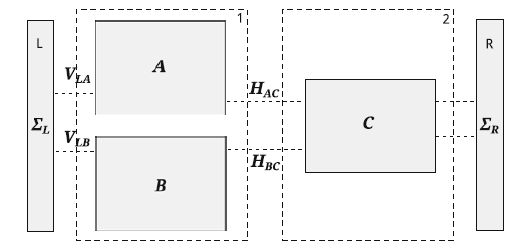
\includegraphics[width=0.7\linewidth]{../figures/multiconnectedgreen.png}
		\label{fig:multiconnectedgreen}
	\end{figure}
	\begin{equation}
		\begin{aligned}
			  & \left( \begin{matrix}
			   {{G}_{A}} & {{G}_{AB}} & {{G}_{AC}}  \\
			   {{G}_{BA}} & {{G}_{B}} & {{G}_{BC}}  \\
			   {{G}_{LA}} & {{G}_{LB}} & {{G}_{L}}  \\
			\end{matrix} \right)=\left( \begin{matrix}
			   G_{A}^{0} & 0 & 0  \\
			   0 & G_{B}^{0} & 0  \\
			   0 & 0 & G_{L}^{0}  \\
			\end{matrix} \right)+ \\ 
			 & \left( \begin{matrix}
			   G_{A}^{0} & 0 & 0  \\
			   0 & G_{B}^{0} & 0  \\
			   0 & 0 & G_{L}^{0}  \\
			\end{matrix} \right)\left( \begin{matrix}
			   0 & 0 & {{V}_{AL}}  \\
			   0 & 0 & {{V}_{BL}}  \\
			   {{V}_{LA}} & {{V}_{LB}} & 0  \\
			\end{matrix} \right)\left( \begin{matrix}
			   {{G}_{A}} & {{G}_{AB}} & {{G}_{AC}}  \\
			   {{G}_{BA}} & {{G}_{B}} & {{G}_{BC}}  \\
			   {{G}_{LA}} & {{G}_{LB}} & {{G}_{L}}  \\
			\end{matrix} \right). \\ 
		\end{aligned}
		\label{eq:expandmultigrren}
	\end{equation}
\end{frame}
\begin{frame}{text here}
	\begin{equation}
		\left( \begin{matrix}
			   {{\Sigma }_{AA}} & {{\Sigma }_{AB}}  \\
			   {{\Sigma }_{BA}} & {{\Sigma }_{BB}}  \\
			\end{matrix} \right)=\left( \begin{matrix}
			   {{V}_{AL}}G_{L}^{0}{{V}_{LA}} & {{V}_{AL}}G_{L}^{0}{{V}_{LB}}  \\
			   {{V}_{BL}}G_{L}^{0}{{V}_{LA}} & {{V}_{BL}}G_{L}^{0}{{V}_{LB}}  \\
			\end{matrix} 
		\right).
	\end{equation}
	\begin{equation}
		{{G}_{C}}={{\left[ E-{{H}_{C}}-{{\Sigma }_{R}}-{{H}_{CA}}G_{A}^{\to (1)}\ {{H}_{AC}}-{{H}_{CB}}G_{B}^{\to (1)}\ {{H}_{BC}} \right]}^{-1}}.
	\end{equation}
\end{frame}
\begin{frame}{text here}
	\begin{equation}
		\begin{aligned}
			&{{A}^{(0)}}={{H}_{1}},\\
			&{{B}^{(0)}}=H_{1}^{\dagger},\\
			&{{C}^{(0)}}=E-{{H}_{0}},\\
			&{{D}^{(0)}}=E-{{H}_{0}},
		\end{aligned}
	\end{equation}
	\begin{equation}
		\begin{aligned}
			&{{A}^{(n)}}={{A}^{(n-1)}}{{({{D}^{(n-1)}})}^{-1}}{{A}^{(n-1)}},\\
			&{{B}^{(n)}}={{B}^{(n-1)}}{{({{D}^{(n-1)}})}^{-1}}{{B}^{(n-1)}},\\
			&{{C}^{(n)}}={{C}^{(n-1)}}-{{A}^{(n-1)}}{{({{D}^{(n-1)}})}^{-1}}{{B}^{(n-1)}},\\
			&{{D}^{(n)}}={{D}^{(n-1)}}-{{A}^{(n-1)}}{{({{D}^{(n-1)}})}^{-1}}{{B}^{(n-1)}}-{{B}^{(n-1)}}{{({{D}^{(n-1)}})}^{-1}}{{A}^{(n-1)}},
		\end{aligned}
	\end{equation}

\end{frame}
%---end section----
\section{Results}
\begin{frame}{Reslt and Disscutions}
	Reslt and Disscutions
\end{frame}
%---begin subsection----
\subsection{text here}
\begin{frame}{borophene}
	\begin{figure}[!ht]
		\centering
		  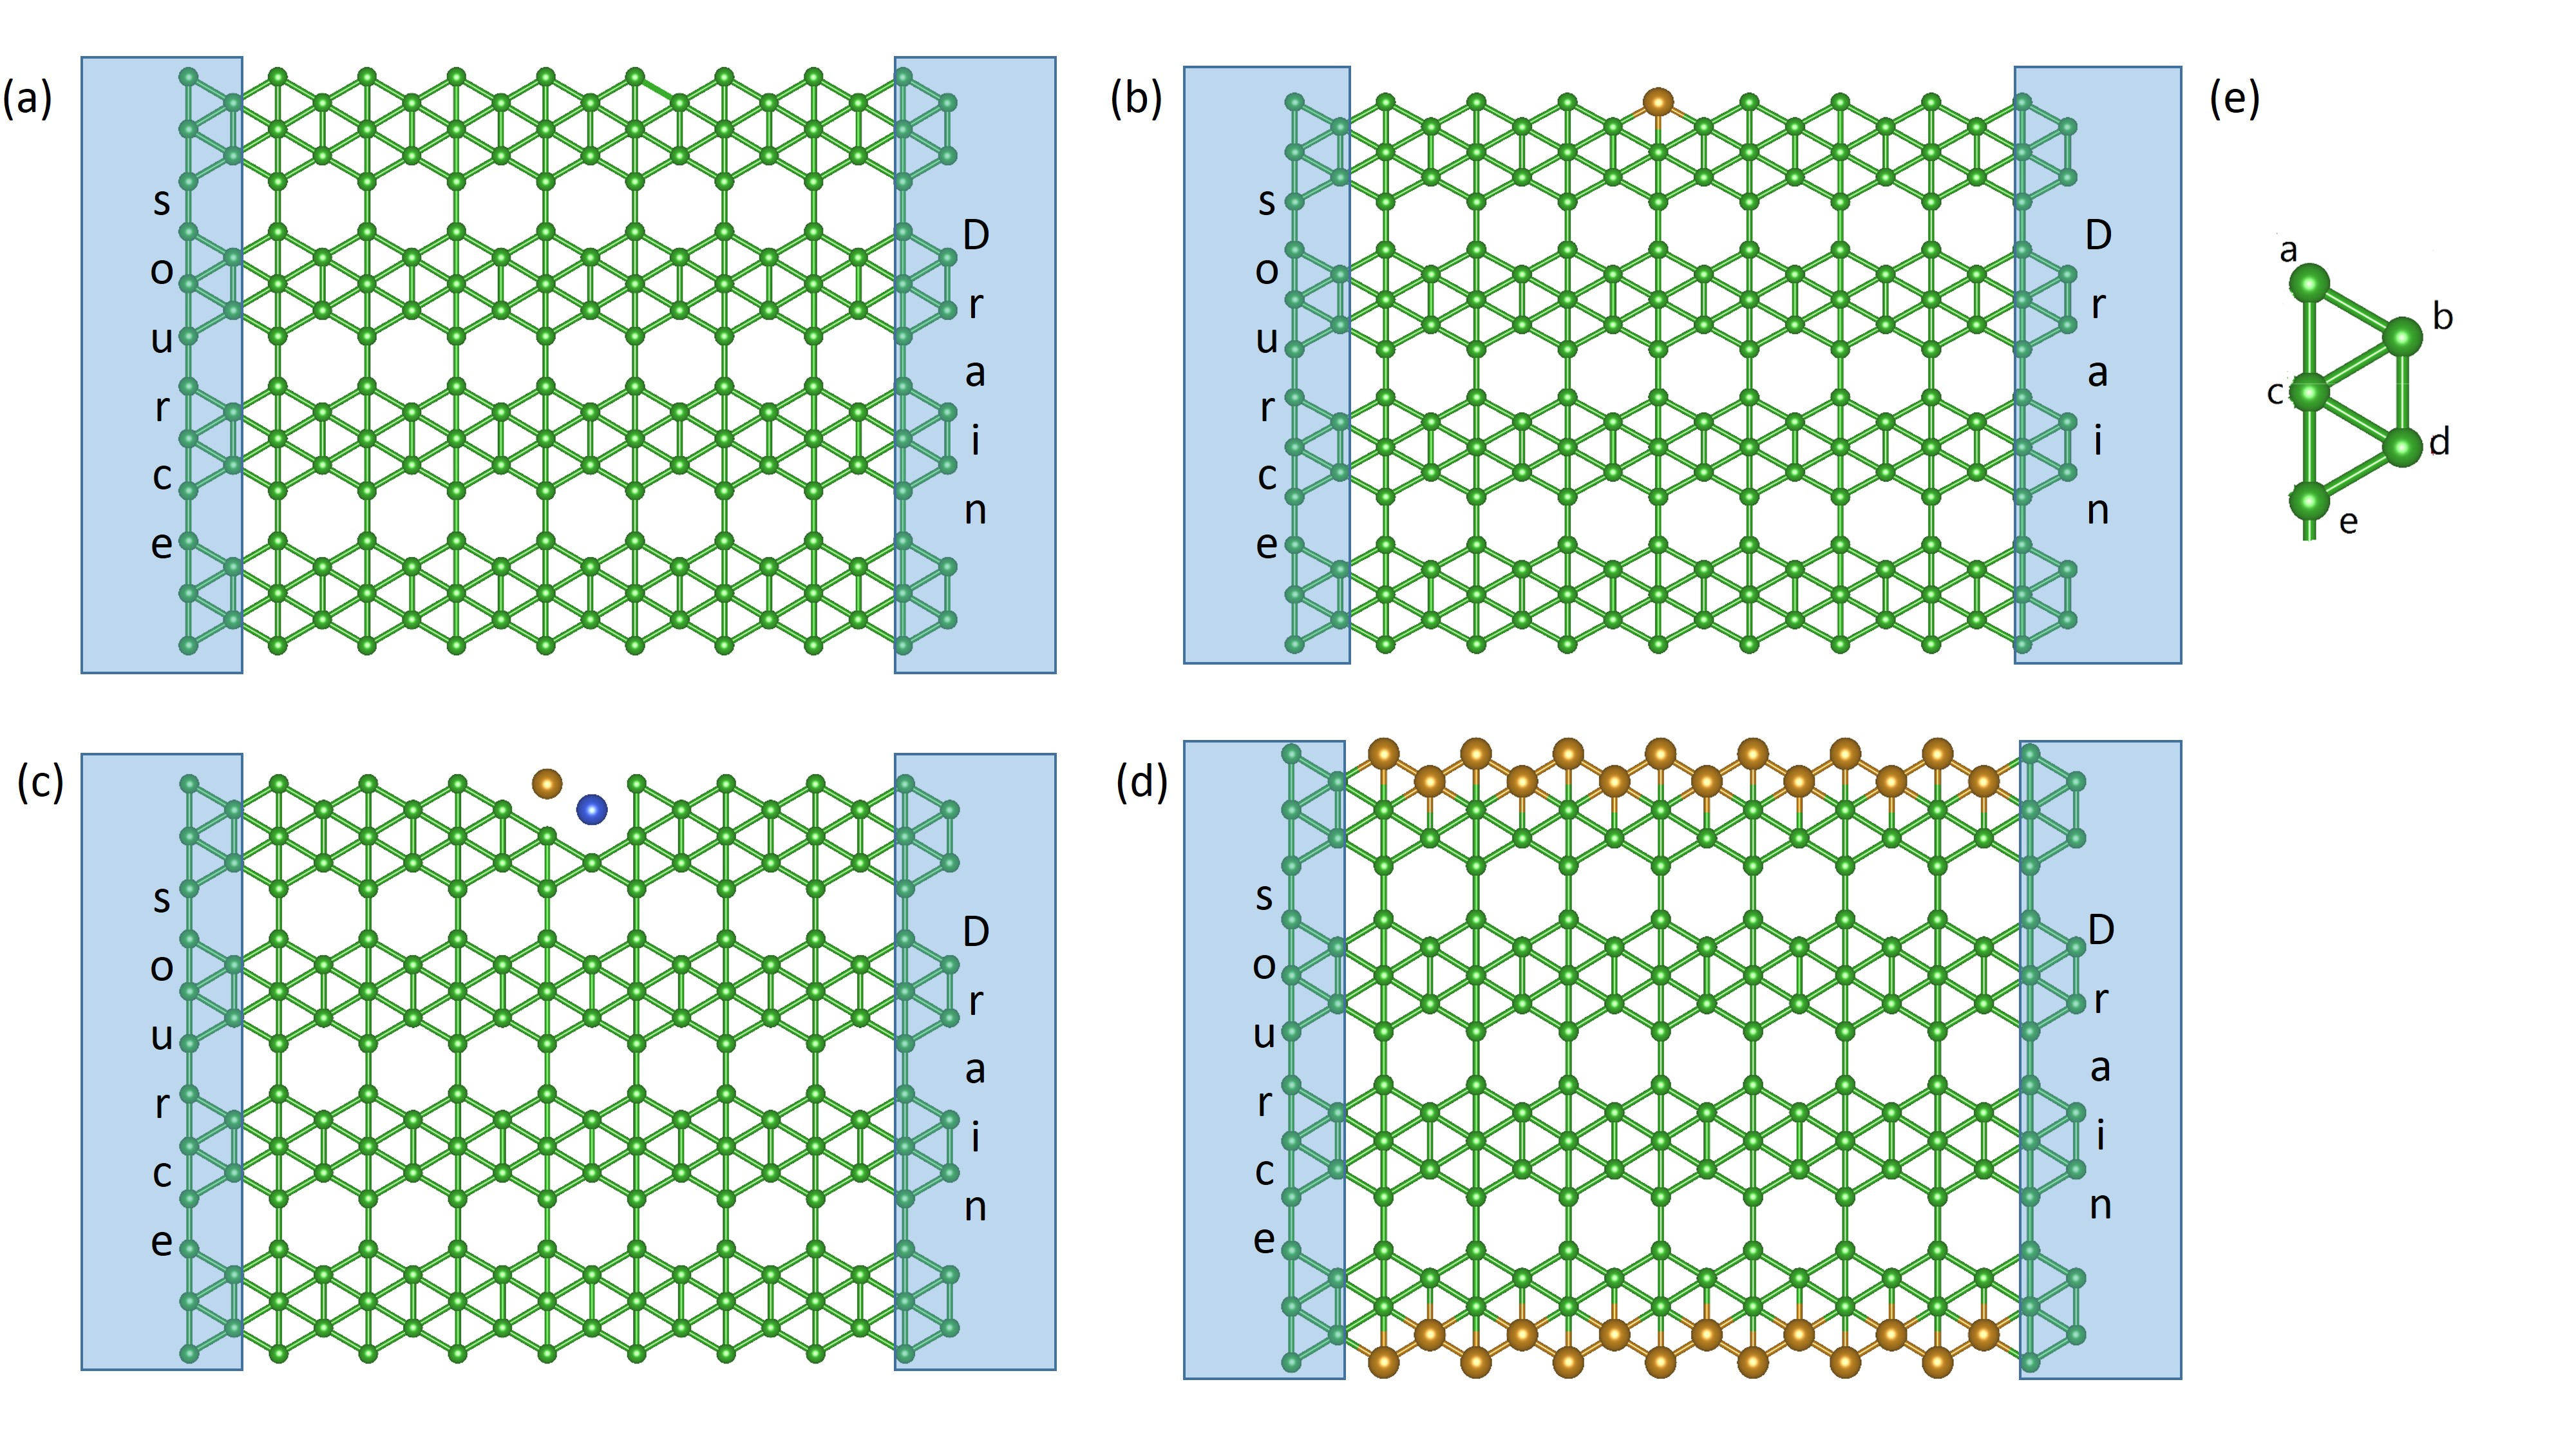
\includegraphics[width=0.8\linewidth]{../figures/borophene_structure(3).JPG}
		 \label{fig:borophene}
	  \end{figure}
\end{frame}

\begin{frame}{zigscatter}
	\begin{figure}[!h]
		\centering
		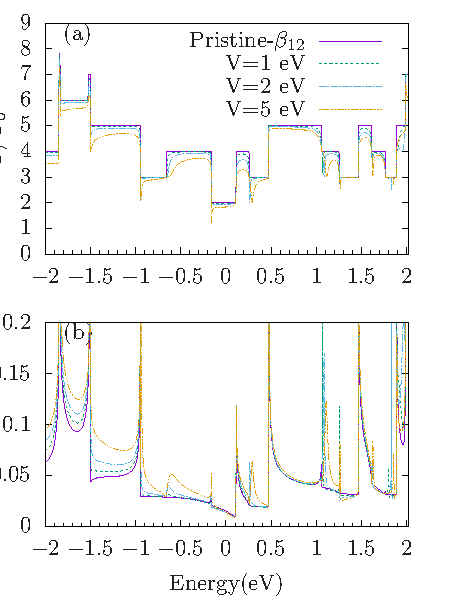
\includegraphics[width=0.5\linewidth]{../figures/zigscatter-thesis.eps}
		\label{zigscatter}
	  \end{figure}
\end{frame}

\begin{frame}{armscatter}
	\begin{figure}[ht]
		\centering
		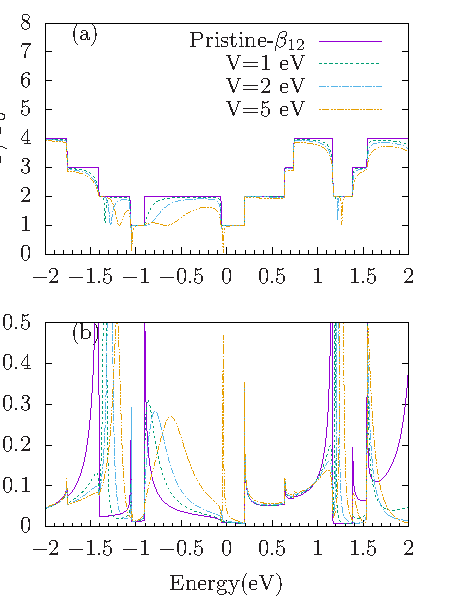
\includegraphics[width=.5\linewidth]{../figures/armscatter-thesis.eps}
		\label{armscatter}
	  \end{figure}
\end{frame}
\begin{frame}{zigvacancy}
	\begin{figure}[ht]
		\centering
		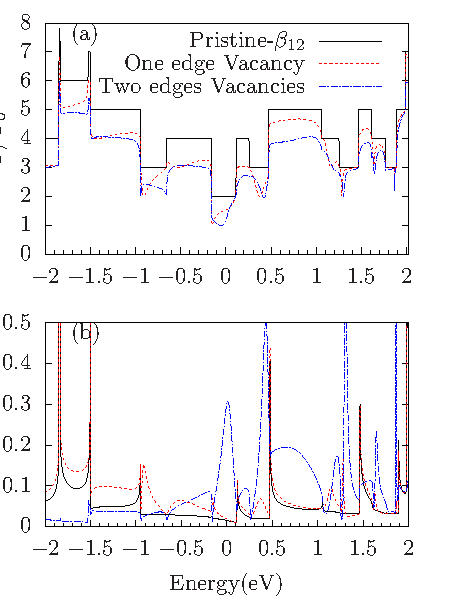
\includegraphics[width=.5\linewidth]{../figures/zigvacancy-thesis.eps}
		\label{zigvacancy}
	  \end{figure}
\end{frame}
\begin{frame}{armvacancy}
	\begin{figure}[ht]
		\centering
		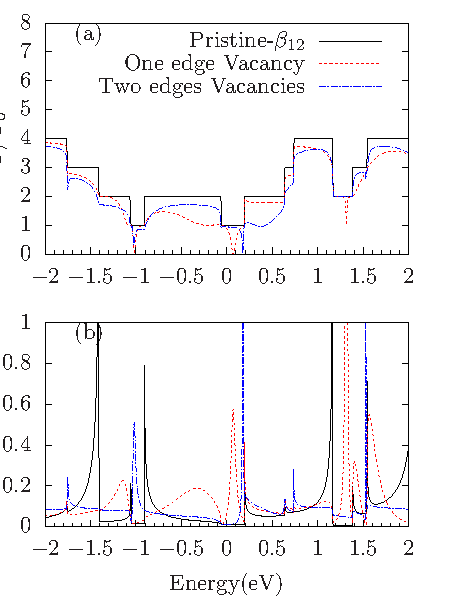
\includegraphics[width=.5\linewidth]{../figures/armvacancy-thesis.eps}
	  \end{figure}
\end{frame}

\begin{frame}{zigzagdisorder}
	\begin{figure}[ht]
		\centering
		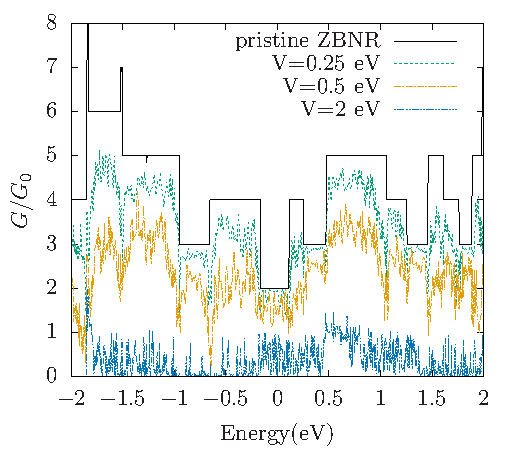
\includegraphics[width=.5\linewidth]{../figures/zigzagdisorder-thesis.eps}
	  \end{figure}
\end{frame}

\begin{frame}{armdisorder}
	\begin{figure}[ht]
		\centering
		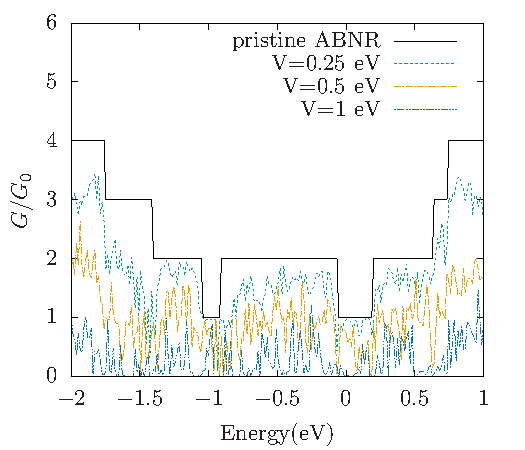
\includegraphics[width=.5\linewidth]{../figures/armdisorder-thesis.eps}
	  \end{figure}
\end{frame}

\begin{frame}{zigzag-width-strangth}
	\begin{figure}[ht]
		\centering
		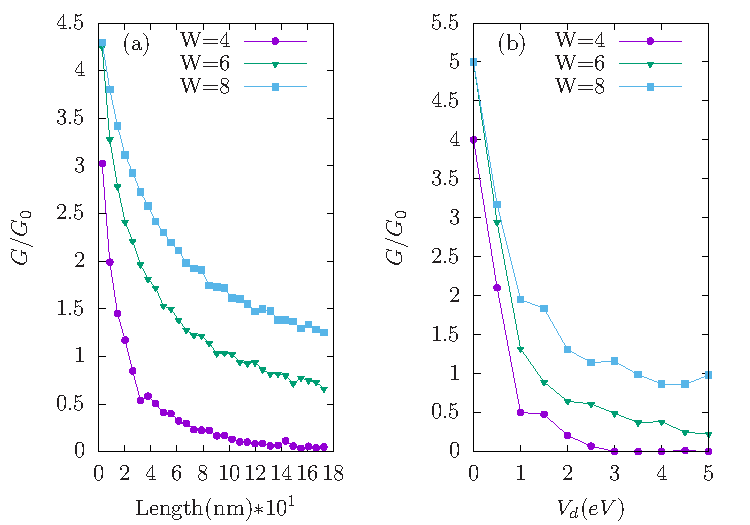
\includegraphics[width=0.5\linewidth]{../figures/zigzag-width-strangth-thesis.eps}
	  \end{figure}
\end{frame}

\begin{frame}{armchair-width-strangth}
	\begin{figure}[ht]
		\centering
		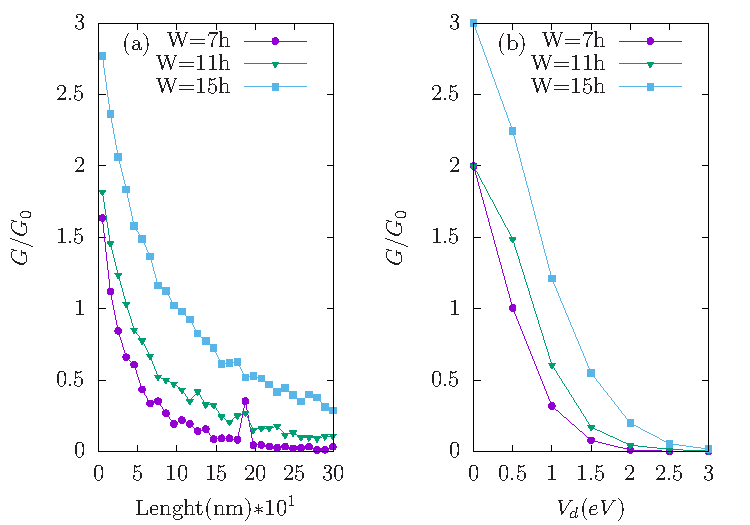
\includegraphics[width=.5\linewidth]{../figures/armchair-width-strangth-thesis.eps}
	  \end{figure}
\end{frame}


\begin{frame}{antiparallel-conductance}
	\begin{figure}
		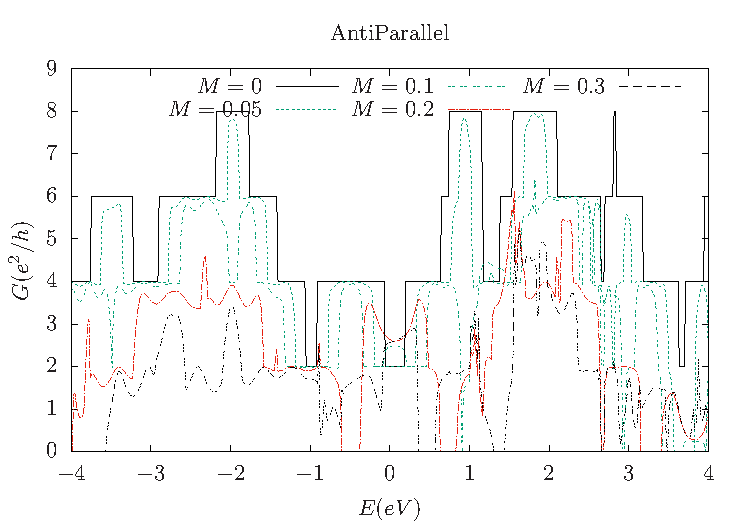
\includegraphics[width=.45\linewidth]{../figures/armchair-antiparallel-conductance-revise-thesis.eps}
		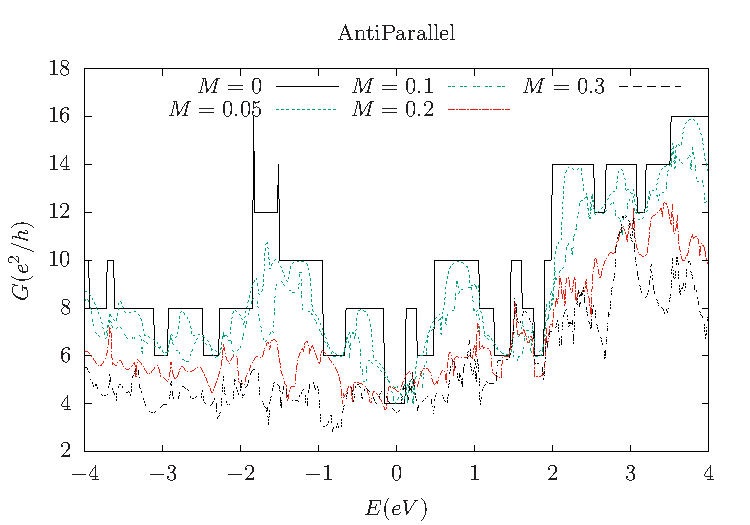
\includegraphics[width=.45\linewidth]{../figures/zigzag-antiparallel-conductance-revise-thesis.eps}
	  \end{figure}
\end{frame}


\begin{frame}{parallel-conductance}
	\begin{figure}[ht]
		\centering
		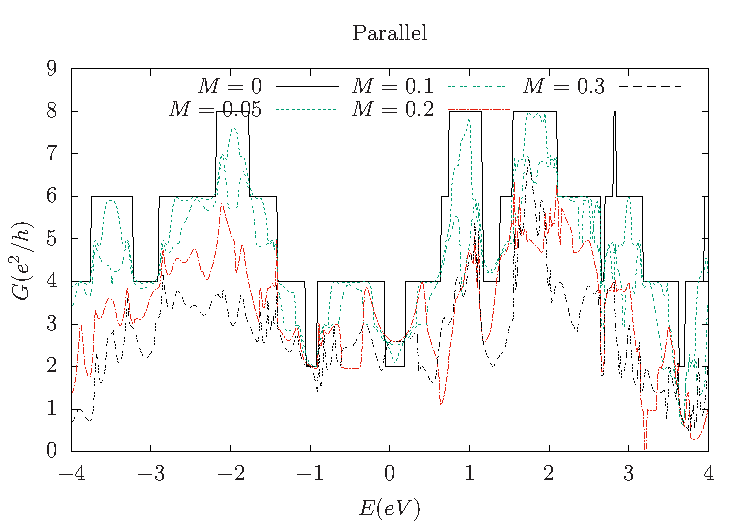
\includegraphics[width=.45\linewidth]{../figures/armchair-parallel-conductance-revise-thesis.eps}
		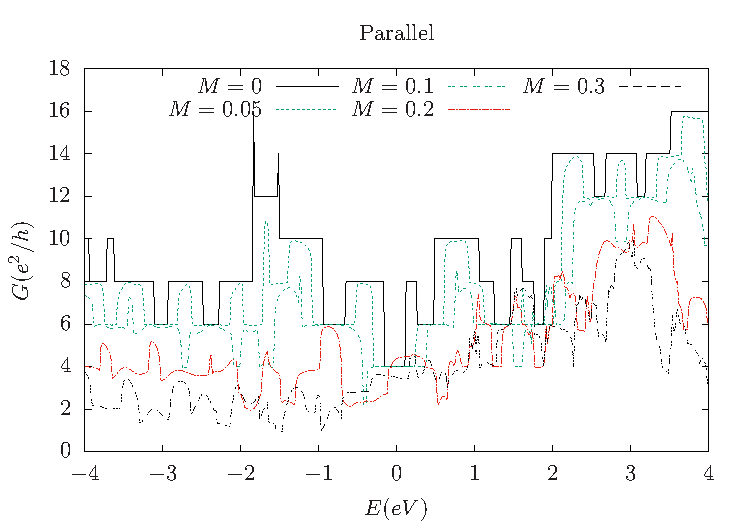
\includegraphics[width=.45\linewidth]{../figures/zigzag-parallel-conductance-revise-thesis.eps}
	  \end{figure}
\end{frame}

\begin{frame}{parallel-conductance}
	\begin{figure}[ht]
		\centering
		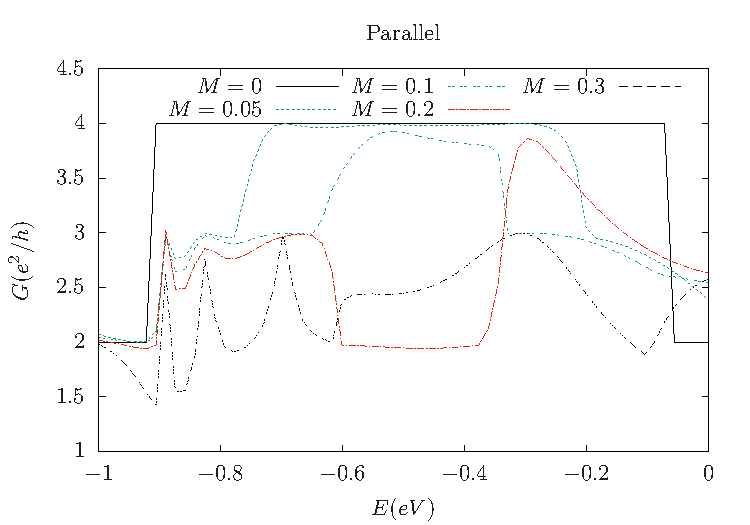
\includegraphics[width=0.45\linewidth]{../figures/armchair-parallel-conductance-1to0-revise-thesis.eps}
		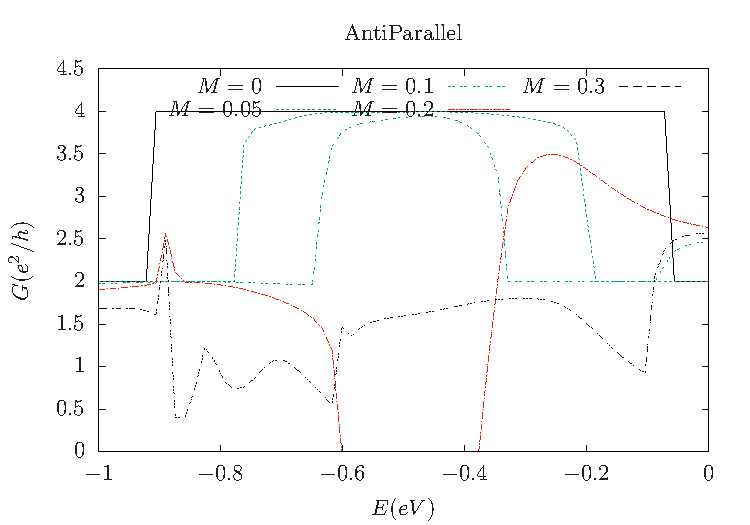
\includegraphics[width=0.45\linewidth]{../figures/armchair-antiparallel-conductance-1to0-revise-thesis.eps}
	  \end{figure}
\end{frame}

\begin{frame}{bandstructure}
	\begin{figure}[ht]
		\centering
		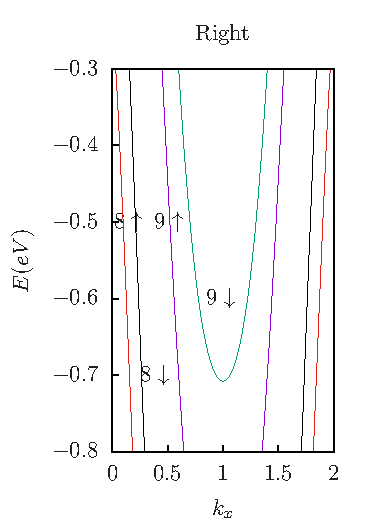
\includegraphics[width=0.33\linewidth]{../figures/Rborophene_band-revised-thesis.eps}
		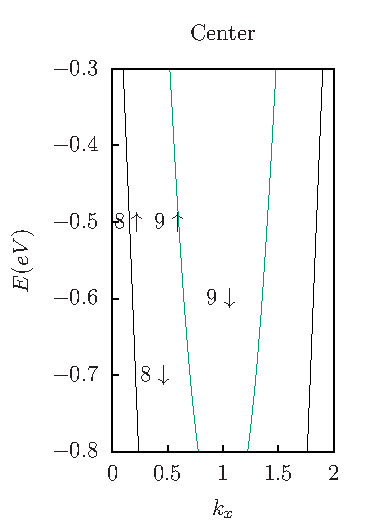
\includegraphics[width=0.33\linewidth]{../figures/Cborophene_band-revised-thesis.eps}
		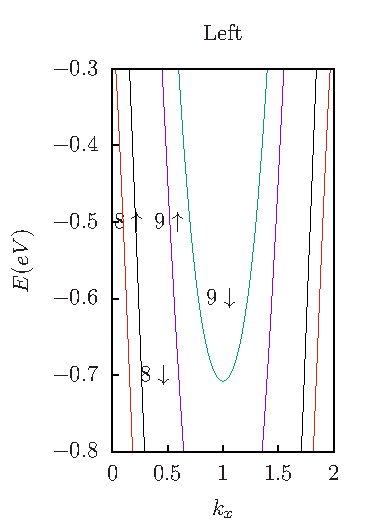
\includegraphics[width=0.33\linewidth]{../figures/Lborophene_band-revised-thesis.eps}
	  \end{figure}
\end{frame}

\begin{frame}{MR}
	\begin{figure}[ht]
		\centering
		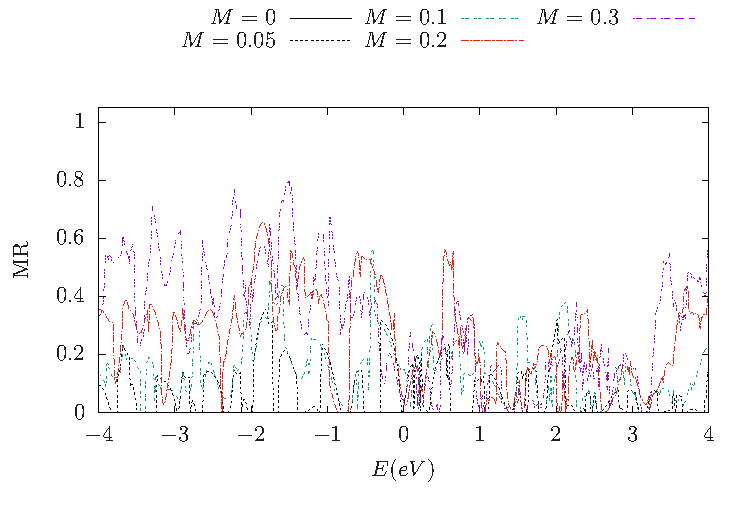
\includegraphics[width=0.45\linewidth]{../figures/MR_zig-revise-thesis.eps}
		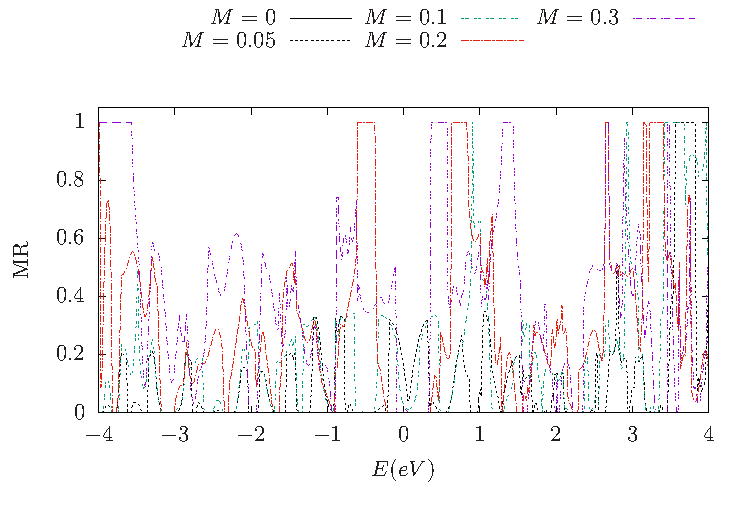
\includegraphics[width=0.45\linewidth]{../figures/MR-revise-thesis.eps}
	  \end{figure}
\end{frame}

\begin{frame}{bandstructure}
	\begin{figure}[ht]
		\centering
		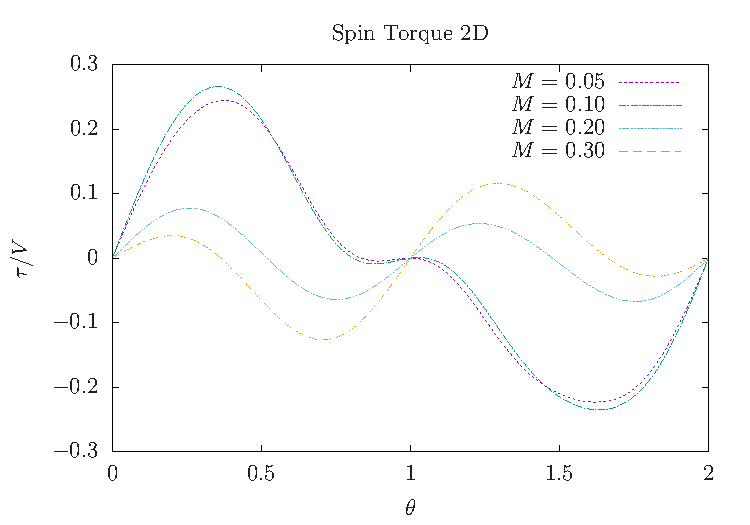
\includegraphics[width=0.45\linewidth]{../figures/stt-thesis.eps}
	  \end{figure}
\end{frame}

\begin{frame}{bandstructure}
	\begin{figure}[ht]
		\centering
		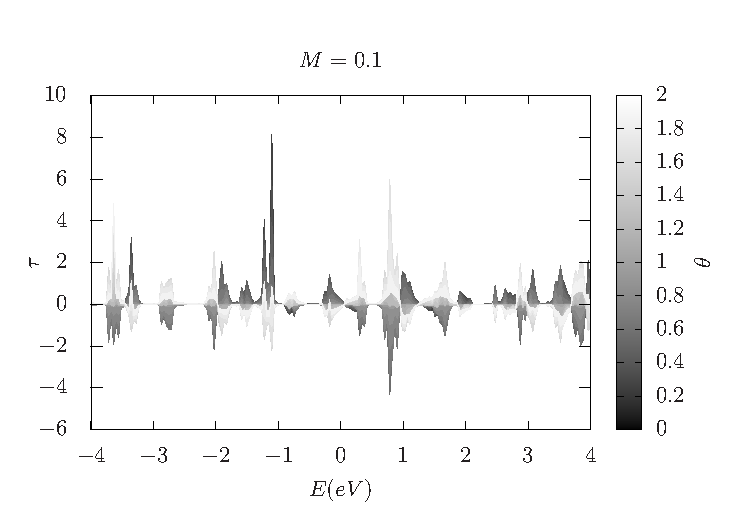
\includegraphics[width=0.33\linewidth]{../figures/stt-energy3d-01-thesis.eps}
		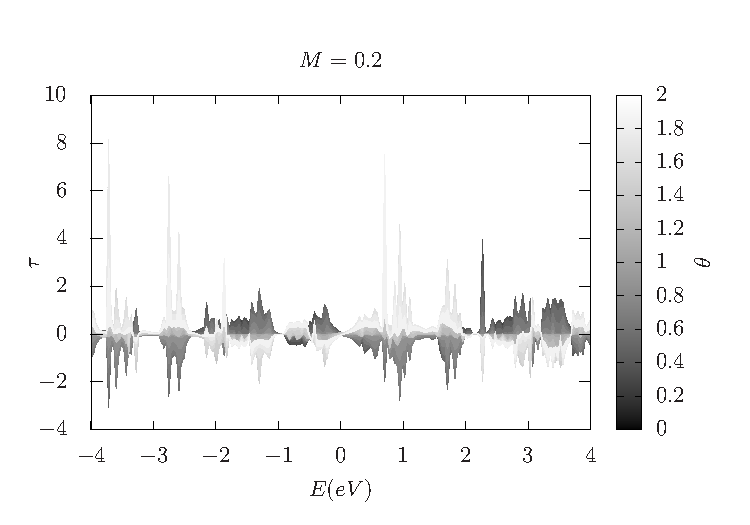
\includegraphics[width=0.33\linewidth]{../figures/stt-energy3d-02-thesis.eps}
		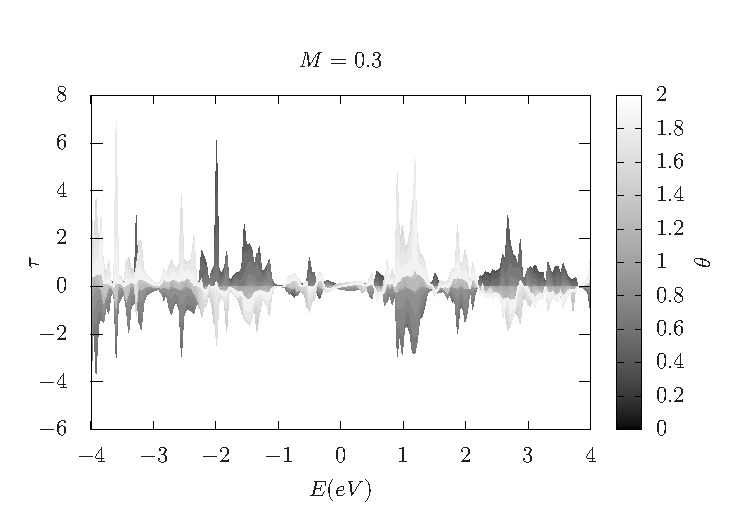
\includegraphics[width=0.33\linewidth]{../figures/stt-energy3d-03-thesis.eps}
	  \end{figure}
\end{frame}


%end subsection
%-------------- Begin references
\section{References}
\begin{frame}{References}
\begin{itemize}
\item $1^{st}$ reference
\end{itemize}
\end{frame}
%------End references-----

\end{document}
